\documentclass{beamer}
\usetheme{metropolis}
\usepackage{graphicx}
\usepackage{subfig}
\usepackage{tcolorbox}
\title{Algebra-Based Physics-2: Electricity, Magnetism, and Modern Physics (PHYS135B-01): Unit 2}
\author{Jordan Hanson}
\institute{Whittier College Department of Physics and Astronomy}

\begin{document}
\maketitle

\section{Unit 1 Review}

\begin{frame}{Unit 1 Review}
\textbf{Reading: Chapters 18 and 19}
\begin{enumerate}
\item Charge, mass, the Coulomb force, and the gravitational force
\item Force fields
\item Electric potential and capacitance
\end{enumerate}
\end{frame}

\section{Unit 1 Review Problems}

\begin{frame}{Unit 1 Review Problems}
\small
\alert{Charged black holes}: Suppose two black holes with the same mass are pulled towards each other by gravity.  Each, however, has a slight positive charge.  If the Coulomb force balances with gravity, what is the charge of the black holes?  Each black hole has a mass of $6 \times 10^{30}$ kg, $G = 7 \times 10^{-11}$ m$^3$ s$^{-2}$ kg$^{-1}$, and $\epsilon_0 = 9\times 10^{-12}$ N$^{-1}$ m$^{-2}$ C$^{2}$.
\begin{itemize}
\item A: $5 \times 10^{40}$ C
\item B: $5 \times 10^{30}$ C
\item C: $5 \times 10^{20}$ C
\item D: $5 \times 10^{10}$ C
\end{itemize}
\textit{Is this number surprisingly small, or surprisingly large?}
\end{frame}

\section{Summary}

\begin{frame}{Unit 2 Summary}
\textbf{Reading: Chapters 20 and 21}
\begin{enumerate}
\item Current, Ohm's Law, resistors and conductors
\item DC circuits I
\item Nerve signals
\item \alert{DC circuits II}
\end{enumerate}
\end{frame}

\section{JITT - Reading Quiz Results}

\begin{frame}{JITT 1.3}
\begin{enumerate}
\item In your own words, make an analogy between current flowing through resistors and water flowing through rivers and dams.
\item What is the difference between resistance and resistivity?
\item Two resistors in series R1 and R2 add like R1+R2.  How is this different from capacitors?
\end{enumerate}
\end{frame}

\begin{frame}{JITT 1.3}
The relationship between resistor and current is that if there is higher resistance, it produces a lower current and if there is lower resistance, it produces a higher current.  In addition, current flowing through resistance is analogous with water flowing through rivers and dams. As the river or dam has lower resistance, avoiding the rocks or branches on the water, the current of the water would be higher than if it contained things that blocked the water from flowing.
\begin{itemize}
\item What is correct?  What needs fixing?
\end{itemize}
\end{frame}

\begin{frame}{JITT 1.3}
Resistance is the specific number of omhs that a conductor has, and it has to do with its shape and the material it is made of. Resistivity is the electrical property of a material.
\begin{itemize}
\item What is correct?  What needs fixing?
\end{itemize}
\end{frame}

\begin{frame}{JITT 1.3}
While resistors add up like R1 + R2, Capacitors add up like 1/R1 + 1/R2.  \\ \vspace{0.5cm}
The sum of the two resistors can just be added up independently along one another as given in the question. When adding capacitors in problems, the likely sum would be in a fraction form. Therefore, adding capacitors compared to adding resistors is a different process.  
\begin{itemize}
\item What is correct?  What needs fixing?
\end{itemize}
\end{frame} 

\section{Current}

\begin{frame}{Current}
\underline{Notions of current:}
\begin{itemize}
	\item $I = \frac{\Delta Q}{\Delta t}$ - The derivative of charge
	\item The \textit{movement} of electrons
	\item The \textit{flow} of charge
	\item Number of Coulombs per second (1 Amp = C/s)
\end{itemize}
\underline{There is an interesting problem with the notion of current} \underline{as movement of charges.} \\ \vspace{0.5cm}
\begin{columns}[T]
\begin{column}{0.5\textwidth}
Speed of typical electronic signals: $\approx 10^{8}$ m/s
\end{column}
\begin{column}{0.5\textwidth}
Typical speed of actual charges passing through a conductor under voltage: $\approx 10^{-4}$ m/s
\end{column}
\end{columns} \vspace{0.25cm}
\textbf{Since there is a 12 order of magnitude range, it's probably a good idea to ponder...}
\end{frame}

\begin{frame}{Current}
\small
Are the electrons colliding/interacting to form electrical signals?  Or just moving all together?
\begin{figure}
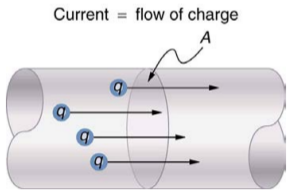
\includegraphics[width=0.5\textwidth]{figures/current1.png}
\caption{\label{fig:current1} The \textit{drift velocity} is the average velocity of an electron, and current is derived from this average velocity.}
\end{figure}
\url{https://youtu.be/8dgyPRA86K0}
\end{frame}

\begin{frame}{Current}
So we see how electrical signals can move near the speed of light, but we measure the movements of electrons in circuits to be slow.  Can we make a calculation to understand the speed of the electrons? \\ \vspace{0.5cm}
\begin{figure}
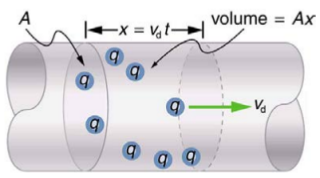
\includegraphics[width=0.5\textwidth]{figures/current3.png}
\caption{\label{fig:current3} Consider the volume $V$ of conductor with cross-sectional area $A$ and length $\Delta x$, having $n$ free electrons per unit volume.}
\end{figure}
\end{frame}

\begin{frame}{Current}
An \textbf{amp} is one \textit{Coulomb} per \textit{second}.  The definition of current is
\begin{equation}
I = \frac{\Delta Q}{\Delta t} = \frac{qnA\Delta x}{\Delta t} = q n A v_{\rm d}
\end{equation}
Solving for drift velocity:
\begin{equation}
v_{\rm d} = \frac{I}{q n A}
\end{equation}
Suppose our conductor is a wire with radius $r$ and $A = \pi r^2$.  Substituting,
\begin{equation}
v_{\rm d} = \frac{I}{\pi q n r^2}
\end{equation}
Remember that $q = 1.6 \times 10^{-19}$ C, and $n$ is the number of free electrons \textit{per atom per unit volume}.  How do we get this number?
\end{frame}

\begin{frame}{Current}
\textbf{Number density}: The total number of objects in a system is equal to the \textit{number density} times the volume of the system.
\begin{equation}
N = nV
\end{equation}
\begin{itemize}
\item N: Total number
\item n: \textit{number density}
\item V: Volume
\end{itemize}
\end{frame}

\begin{frame}{Current}
\textbf{Example:} \alert{Number of Stars in the Milky Way}.  How many stars are in our galaxy?  Assume the galaxy is a disk of height $h$ and radius $r$.  We observe $n$ stars per unit volume.
\begin{itemize}
\item $r$ = $50 \times 10^3$ \textit{light-years}
\item $h = 2 \times 10^3$ \textit{light-years}
\item $n = 10^{-2}$ \textit{light-year} $^{-3}$
\end{itemize}
\begin{enumerate}
\item Compute the volume in \textit{light-years}$^3$
\item Multiply the volume by the number density to obtain the total number.
\item Compare the result with others' results.
\end{enumerate}
\end{frame}

\begin{frame}{Current}
\small
How many \textbf{conduction} electrons are there in a cube of copper that is 1 micron (1 $\mu$m = $10^{-6}$ m) on a side?
\begin{itemize}
\item Copper has a density of 8.8 grams per cubic centimeter.
\item Copper has an atomic weight of 63.54 grams per mole.  (\textit{Do you remember what a mole is?}).
\item There are $N_A = 6.02 \times 10^{23}$ atoms per mole.
\item Only one electron per atom of copper is a conduction electron.
\end{itemize} \hrulefill
\begin{enumerate}
\item Divide the density by the atomic weight.  What are the units?
\item Multiply by $N_A$ (Avogadro's number).  What are the units?
\item Convert the units from $cm^{-3}$ to $\mu m^{-3}$.
\end{enumerate}
\end{frame}

\begin{frame}{Current}
\textbf{Number density}: Let's examine copper, a common wire material with one free electron per atom.  Copper has a density of 8800 kg/m$^3$, and $0.06354$ kg/mol.  There are $6.02 \times 10^{23}$ atoms/mol.  How many free electrons per m$^3$ of copper? (Remember that there is only one conduction electron per copper atom).
\begin{itemize}
\item A: $8.34 \times 10^{26}$ free electrons per m$^3$
\item B: $8.34 \times 10^{27}$ free electrons per m$^3$
\item C: $8.34 \times 10^{28}$ free electrons per m$^3$
\item D: $8.34 \times 10^{29}$ free electrons per m$^3$
\end{itemize}
\end{frame}

\begin{frame}{Current}
Consider a copper wire with radius $r = 2.053$ mm that is carrying 20.0 A of current.  Using $q = 1.6\times 10^{19}$, and $n = 8.34 \times 10^{28}$ electrons/m$^3$, and $v_{\rm d} = I/(\pi q n r^2)$, compute the drift velocity of charge in the wire.  \textit{This is a common situation in household wiring.}
\begin{itemize}
\item A: $10^{-1}$ m/s
\item B: $10^{-2}$ m/s
\item C: $10^{-3}$ m/s
\item D: $10^{-4}$ m/s
\end{itemize}
\end{frame}

\begin{frame}{Current}
\textbf{Drift speed vs. signal speed}.  Given that the electrons move at 1mm/s, how is it that electric signals move at $10^8$ m/s? \\ \vspace{1cm}
\textbf{Electrical signals are more like a \alert{wave on a string}}: \\ \url{https://phet.colorado.edu/en/simulation/legacy/wave-on-a-string}
\end{frame}

\section{Ohm's Law}

\begin{frame}{Current}
\small
Electrons are now moving through our copper wire ($v_{\rm d} \propto I$, $v_{\rm d} \propto A^{-1}$).  What happens when the electrons, which have had some PE converted to KE, encounter objects that are not conductors?  \textbf{They deposit energy and move forward.} \\ \vspace{0.5cm}
\begin{figure}
\centering
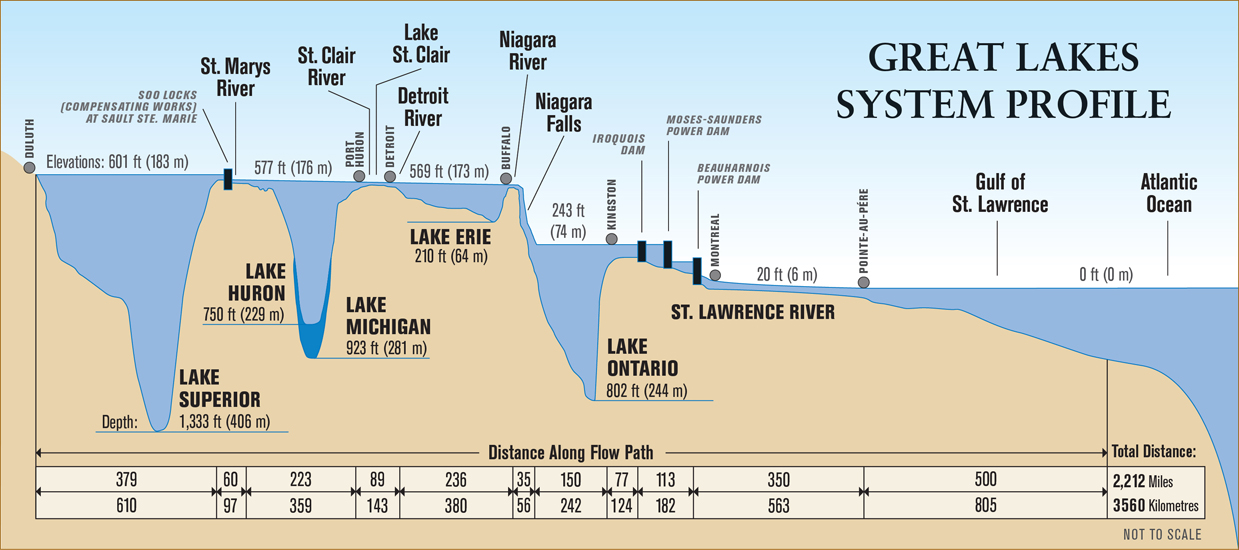
\includegraphics[width=0.5\textwidth]{figures/lakes.jpg}
\caption{\label{fig:lakes} Current is comprised of electrons that deposit energy as they move to lower voltages.}
\end{figure}
\textbf{\alert{PhET}}: \url{https://phet.colorado.edu/en/simulation/circuit-construction-kit-dc}
\end{frame}

\begin{frame}{Current}
\textbf{\alert{PhET}}: Create a DC circuit involving a battery, resistor (the brown striped object), a light bulb, and a switch.
\begin{enumerate}
\item Place the battery and connect to it a wire, and attach a resistor to that wire.
\item To the other end of the resistor, connect a switch and leave it open.
\item Connect a light bulb to the other end of the switch, and connect a wire from the light bulb to the battery.
\item The properties of each circuit element can be edited by clicking on the element.
\end{enumerate}
\end{frame}

\begin{frame}{Current}
\begin{figure}
\centering
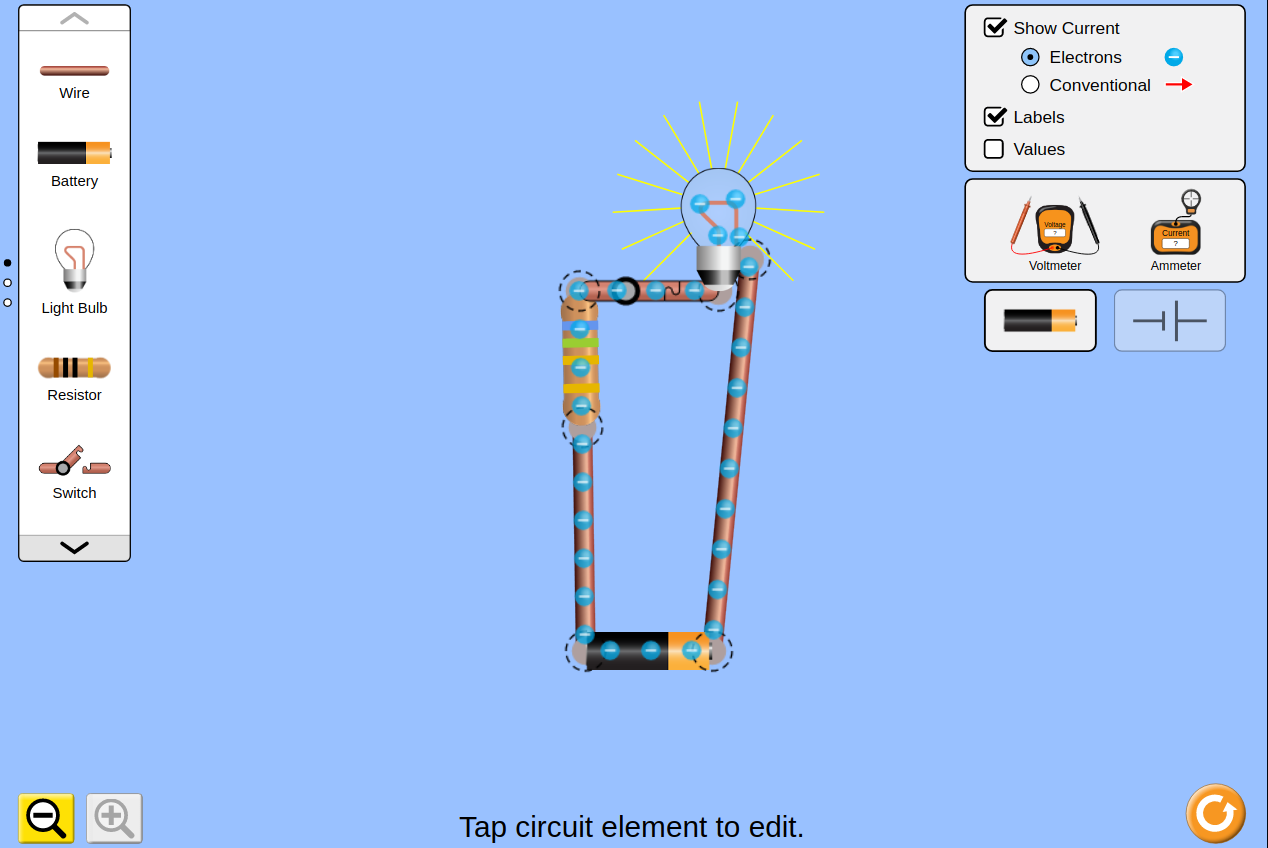
\includegraphics[width=0.75\textwidth]{figures/PhETBulb.png}
\caption{\label{fig:phetb} Your circuit should resemble this.}
\end{figure}
\end{frame}

\begin{frame}{Current}
\textbf{\alert{PhET}}: Make observations.
\begin{enumerate}
\item What happens to the drift velocity of the electrons as you raise and lower the resistance?  Why do we call light bulbs and the brown striped objects ``resistors?''
\item Since we cannot change the cross-sectional area of the wire independently, we can treat $v_{\rm d} \propto I$.
\item How does the current change if you increase the voltage?
\end{enumerate}
\end{frame}

\begin{frame}{Current}
\textbf{\alert{PhET}}: \textbf{The unit of resistance is the Ohm.  We use the symbol $\Omega$ for Ohms, and $1\Omega = 1$V/A.}
\begin{enumerate}
\item There are two devices available: the \textit{voltmeter}, and the \textit{ammeter}.  Using these devices, measure the voltage drop across the resistor and the light bulb, and the current flowing through the circuit.
\item How are voltage and current and resistance related?  Derive an equation from the data.
\end{enumerate}
\end{frame}

\begin{frame}{Current}
\textbf{Ohm's Law}: Let $V$ be the voltage change across a resistor with resistance $R$, and let $i$ be the current flowing through the resistor.  Ohm's law states that
\begin{equation}
\boxed{
V = iR}
\end{equation}
for materials that fall into the category of \textit{Ohmic}.
\end{frame}

\begin{frame}{Current}
\textbf{\alert{PhET}}: \textbf{How do we deal with more complex circuits?} There must be a way to ``add'' resistors.
\begin{enumerate}
\item Create a circuit that involves just a hairy mess of resistors.  Connect them \textit{in series} and \textit{in parallel}.
\item Calculate the \textit{effective total resistance} by plotting an $i-V$ curve of the system.  Measure $i$ and $V$ by changing the voltage and using the voltmeter and ammeter.
\item What is the effective total resistance of the circuit?  How did you obtain this number from the $i-V$ curve?
\end{enumerate}
\end{frame}

\begin{frame}{Current}
As you may have discovered, \textit{resistors in series} \textbf{add}:
\begin{equation}
R_{\rm tot} = R_1 + R_2 + ...
\end{equation}
\textit{Resistors in parallel} \textbf{add their reciprocals}:
\begin{equation}
\frac{1}{R_{\rm tot}} = \frac{1}{R_1}+\frac{1}{R_2}+...
\end{equation}
\end{frame}

\section{JITT 1.4}

\begin{frame}{JITT 1.4}
\begin{enumerate}
\item What are Kirchhoff's two rules for circuits?
\item Consider a DC circuit with two resistors, each having resistance R.  Which circuit has higher resistance: a) the two resistors are connected in series, or b) the two resistors are connected in parallel?
\item Same circuit as (2).  For the in-series case, is the current flowing through each resistor the same?
\end{enumerate}
\end{frame}

\begin{frame}{JITT 1.4}
\textbf{What are Kirchhoff's two rules for circuits?} \\
``The junction rule, which states that the sum of all currents entering a junction must equal the sum of all currents, and The loop rule, which states that the algebraic sum of changes in potential around any closed circuit path must be zero.''
\end{frame}

\begin{frame}{JITT 1.4}
\textbf{Consider a DC circuit with two resistors, each having resistance R.  Which circuit has higher resistance: a) the two resistors are connected in series, or b) the two resistors are connected in parallel?} \\
``In series.''
\end{frame}

\begin{frame}{JITT 1.4}
\textbf{Same circuit as (2).  For the in-series case, is the current flowing through each resistor the same?} \\
``The same.''
\end{frame}

\begin{frame}{Current}
Resitance is not an \textit{intrinsic property} of materials.  Imagine a 0.1 m-long wire (which is a conductor) actually having a small resistance.  What about that same wire, but 1 kilometer long?
\begin{itemize}
\item Electrons lose some fixed energy per unit length in a given material (\textit{Joule heating})
\item Electrons lose more energy if the wire is thinner (\textit{Joule heating})
\end{itemize}
\textbf{Resistivity} $\rho$ is defined in terms of resistance $R$, length $L$ and cross-sectional area $A$ as
\begin{equation}
R = \rho \left( \frac{L}{A} \right)
\end{equation}
\end{frame}

\begin{frame}{Current}
\begin{columns}[T]
\begin{column}{0.5\textwidth}
\begin{figure}
\centering
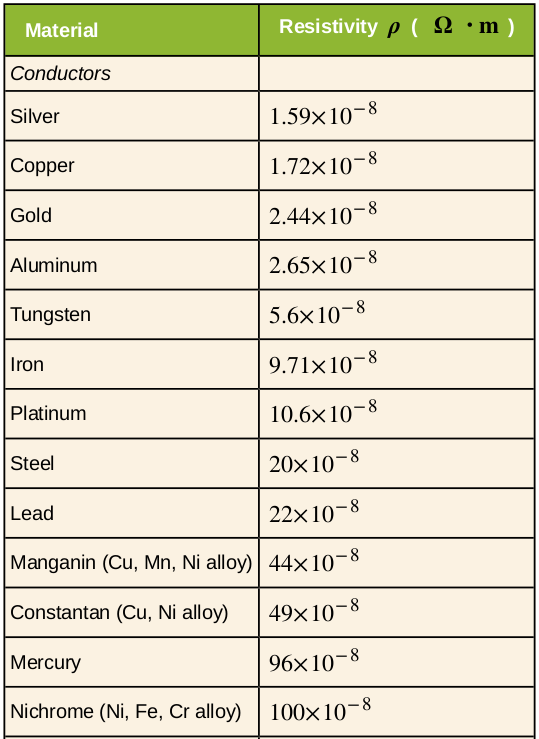
\includegraphics[width=0.7\textwidth]{figures/rho1.png}
\caption{\label{fig:rho1} Conductor resistivities are in units of $\Omega$ m, and are small but non-zero.}
\end{figure}
\end{column}
\begin{column}{0.5\textwidth}
\begin{figure}
\centering
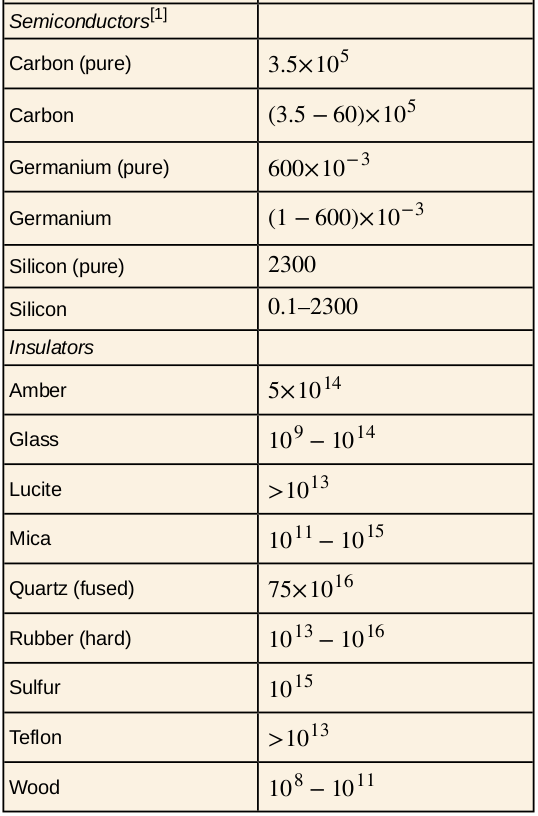
\includegraphics[width=0.7\textwidth]{figures/rho2.png}
\caption{\label{fig:rho2} Semiconductor resistivities are in units of $\Omega$ m, and are larger.}
\end{figure}
\end{column}
\end{columns}
\end{frame}

\begin{frame}{Current}
A copper wire carrying current to the top floor of a building, that has a cross-sectional area of 12 mm$^2$ and is 10 meters long.  The resistivity of copper is $1.7 \times 10^{-8}$ $\Omega$ m.  What is the resistance of the wire?
\begin{itemize}
\item A: about 1 m$\Omega$
\item B: about 10 m$\Omega$
\item C: about 100 m$\Omega$
\item D: about 1 $\Omega$
\end{itemize}
\end{frame}

\begin{frame}{Current}
Consider the same system.  If we attach a battery and use the wire to feed voltage to some circuit drawing 3.0 A of current, what is the voltage drop due to just the wire?
\begin{itemize}
\item A: about 30 mV
\item B: about 300 mV
\item C: about 3 V
\item D: Current will not flow at all
\end{itemize}
\end{frame}

\begin{frame}{Current}
What would the resistance be if the wire system was 10 times as long?
\begin{itemize}
\item A: about 30 mV
\item B: about 300 mV
\item C: about 3 V
\item D: Current will not flow at all
\end{itemize}
\textit{So you can start to see that resistance matters even for conductors, if the current is traveling for long distances.  Often manufacturers quote the Ohms per foot in wire data sheets.}
\end{frame}

\begin{frame}{Current}
Resistivity depends on temperature in the following way:
\begin{equation}
\rho = \rho_{\rm 0} \left(1 + \alpha \Delta T\right)
\end{equation}
For most conductors, $\alpha$ is small, on the order of $10^{-3}$ $^\circ$C$^{-1}$.
\end{frame}

\begin{frame}{Current}
\begin{figure}
\centering
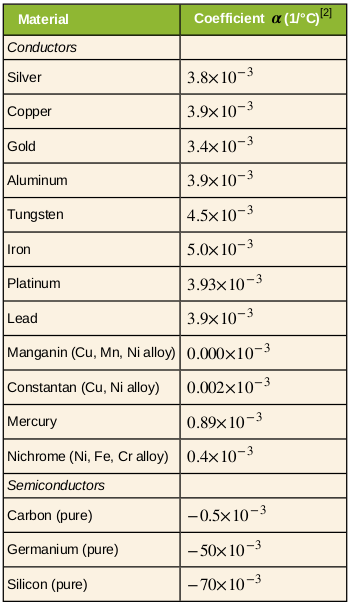
\includegraphics[width=0.35\textwidth]{figures/rho3.png}
\caption{\label{fig:rho3} Conductor resistivities depend on temperature.}
\end{figure}
\end{frame}

\begin{frame}{Current}
Continuing with the same example of the long copper wire with $R = 10$ m$\Omega$, if the temperature increases by 50.0 deg C, what is the new resistance? ($\alpha = 3.9 \times 10^{-3}$ $^{\circ}$C$^{-1}$).
\begin{itemize}
\item A: 8 m$\Omega$
\item B: 12 m$\Omega$
\item C: 18 m$\Omega$
\item D: 22 m$\Omega$
\end{itemize}
\end{frame}

\begin{frame}{Current}
Recall that \textbf{power} is consumed in resistors, since charges are losing energy and new charges are showing up at a certain rate.  Consider the PE converted to work in a resistor:
\begin{align}
\Delta PE =& \Delta q\Delta V \\
\Delta W =& \Delta q i R \\
\frac{\Delta W}{\Delta t} =& \frac{\Delta q}{\Delta t} i R = i^2 R \\
\frac{\Delta W}{\Delta t} =& i V \\
P =& iV
\end{align}
The formula $P = iV$ shows that the wattage required by some device in a circuit will pull current according to the voltage of the battery.
\end{frame}

\begin{frame}{Current}
How much current is required by a 50 W light bulb if the voltage supplying it is 120 V?
\begin{itemize}
\item A: 420 mA
\item B: 120 mA
\item C: 50 mA
\item D: 50 V
\end{itemize}
\end{frame}

\begin{frame}{Current}
\begin{columns}[T]
\begin{column}{0.5\textwidth}
\begin{figure}
\centering
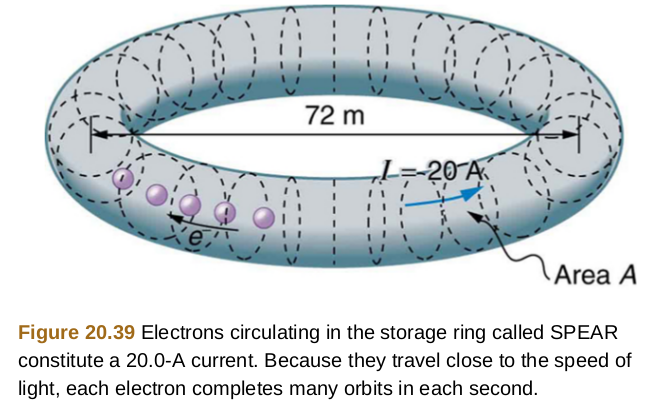
\includegraphics[width=\textwidth]{figures/SPEAR.png}
\caption{\label{fig:SLAC} A component of the Stanford Linear Accelerator (SLAC) stores high-energy electrons.}
\end{figure}
\end{column}
\begin{column}{0.5\textwidth}
\small
SPEAR, a storage ring about 72.0 m in diameter at the Stanford Linear Accelerator (closed in 2009), has a 20.0-A circulating beam of electrons that are moving at nearly the speed of light. (See Figure 20.39.) How many electrons are in the beam?
\begin{itemize}
\item A: $2 \times 10^{11}$
\item B: $2 \times 10^{12}$
\item C: $2 \times 10^{13}$
\item D: $2 \times 10^{14}$
\end{itemize}
\end{column}
\end{columns}
\end{frame}

\begin{frame}{Current}
\begin{columns}[T]
\begin{column}{0.5\textwidth}
\begin{figure}
\centering
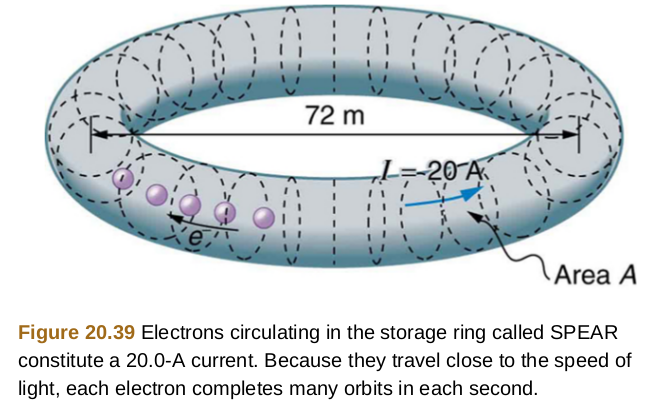
\includegraphics[width=\textwidth]{figures/SPEAR.png}
\caption{\label{fig:SLAC2} A component of the Stanford Linear Accelerator (SLAC) stores high-energy electrons.}
\end{figure}
\end{column}
\begin{column}{0.5\textwidth}
\small
Suppose each electron was dropped through a potential of 1 kV as it enters the ring.  What is the energy of each electron?
\begin{itemize}
\item A: 100 eV
\item B: 1 keV
\item C: 1 MeV
\item D: 1 Joule
\end{itemize}
\end{column}
\end{columns}
\end{frame}

\begin{frame}{Current}
\begin{columns}[T]
\begin{column}{0.5\textwidth}
\begin{figure}
\centering
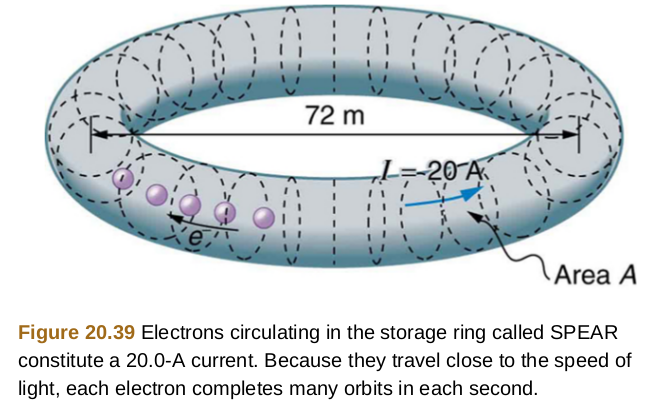
\includegraphics[width=\textwidth]{figures/SPEAR.png}
\caption{\label{fig:SLAC3} A component of the Stanford Linear Accelerator (SLAC) stores high-energy electrons.}
\end{figure}
\end{column}
\begin{column}{0.5\textwidth}
\small
What's the total energy of all the electrons?  (Multiply the previous two answers).
\begin{itemize}
\item A: $2 \times 10^{16}$ eV
\item B: $2 \times 10^{17}$ eV
\item C: $2 \times 10^{18}$ eV
\item D: $2 \times 10^{19}$ eV
\end{itemize}
\end{column}
\end{columns}
\end{frame}

\begin{frame}{Current}
\begin{columns}[T]
\begin{column}{0.5\textwidth}
\begin{figure}
\centering
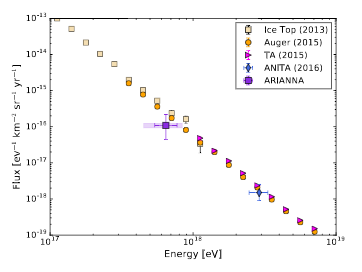
\includegraphics[width=0.9\textwidth]{figures/ARIANNA1.png}
\caption{\label{fig:ARIANNA1} Cosmic ray protons' flux observed recently by the ARIANNA experiment.}
\end{figure}
\end{column}
\begin{column}{0.5\textwidth}
\small
How much energy is $2 \times 10^{17}$ eV?  Recently, the ARIANNA experiment observed protons with so much energy (about $2 \times 10^{17}$ eV) the ensuing shock in the atmosphere created a radio pulse observed over a several kilometer range.
\end{column}
\end{columns}
\end{frame}

\begin{frame}{Current}
\begin{columns}[T]
\begin{column}{0.5\textwidth}
\begin{figure}
\centering
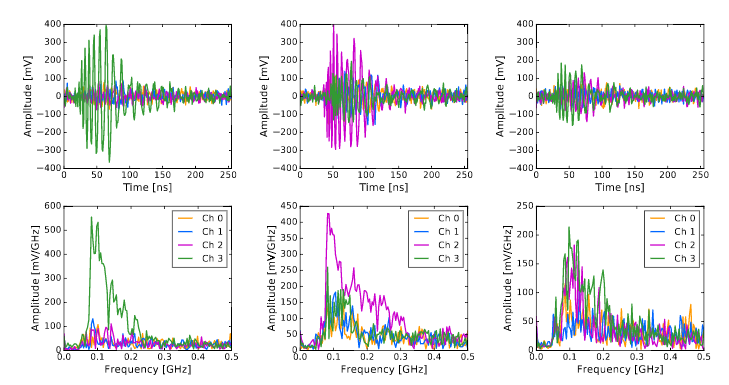
\includegraphics[width=0.9\textwidth]{figures/ARIANNA2.png}
\caption{\label{fig:ARIANNA2} Cosmic ray protons' flux observed recently by the ARIANNA experiment.}
\end{figure}
\end{column}
\begin{column}{0.5\textwidth}
\small
How much energy is $2 \times 10^{17}$ eV?  Recently, the ARIANNA experiment observed protons with so much energy (about $2 \times 10^{17}$ eV) the ensuing shock in the atmosphere created a radio pulse observed over a several kilometer range.
\end{column}
\end{columns}
\end{frame}

\begin{frame}{Current}
\begin{columns}[T]
\begin{column}{0.5\textwidth}
\begin{figure}
\centering
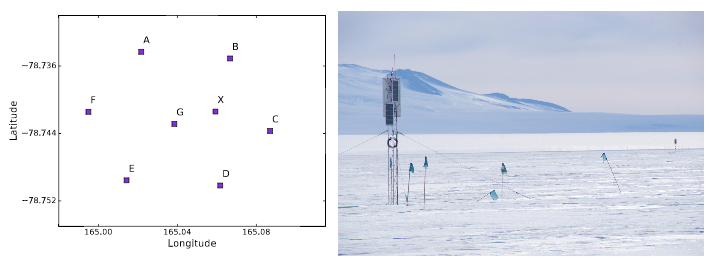
\includegraphics[width=0.9\textwidth]{figures/ARIANNA3.png}
\caption{\label{fig:ARIANNA3} Cosmic ray protons' flux observed recently by the ARIANNA experiment.}
\end{figure}
\end{column}
\begin{column}{0.5\textwidth}
\small
How much energy is $2 \times 10^{17}$ eV?  Recently, the ARIANNA experiment observed protons with so much energy (about $2 \times 10^{17}$ eV) the ensuing shock in the atmosphere created a radio pulse observed over a several kilometer range.
\end{column}
\end{columns}
\textit{Good paper topic:} What is the purpose of the ARIANNA and ARA experiments in the Antarctic?  What are they trying to measure?
\end{frame}

\section{Graphical Analysis of Simple Circuits}

\begin{frame}{Current}
\begin{columns}[T]
\begin{column}{0.5\textwidth}
\begin{figure}
\centering
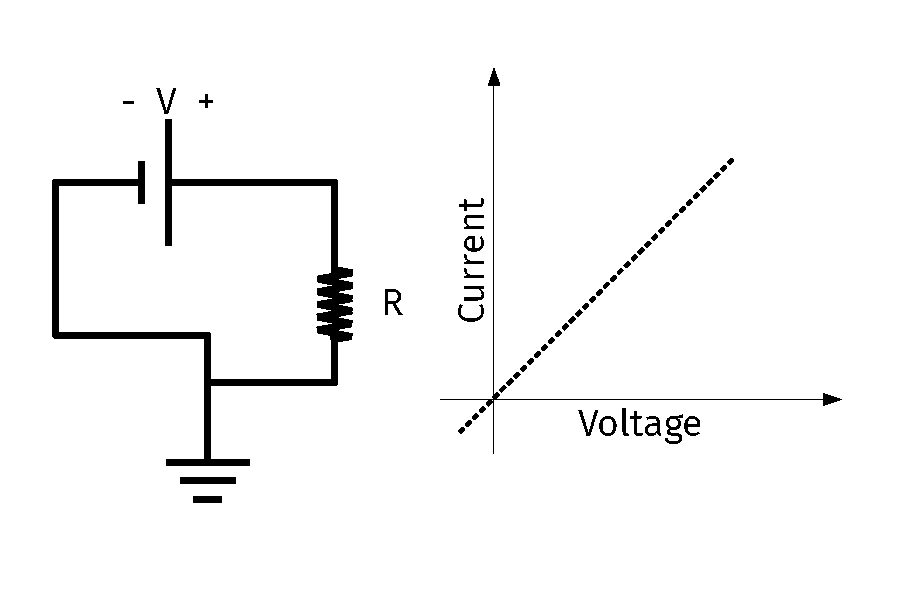
\includegraphics[width=\textwidth,trim=0.5cm 0cm 1cm 0cm,clip=true]{figures/iVCurve.pdf}
\caption{\label{fig:iVCurve1} Circuits components are represented graphically by iV curves.}
\end{figure}
\end{column}
\begin{column}{0.5\textwidth}
\small
If the resistance $R$ is increased, what will happen?
\begin{itemize}
\item A: The slope on the graph will increase
\item B: The slope on the graph will decrease
\item C: The slope will stay the same
\item D: Cannot determine what will happen
\end{itemize}
\end{column}
\end{columns}
\end{frame}

\begin{frame}{Current}
\begin{columns}[T]
\begin{column}{0.5\textwidth}
\begin{figure}
\centering
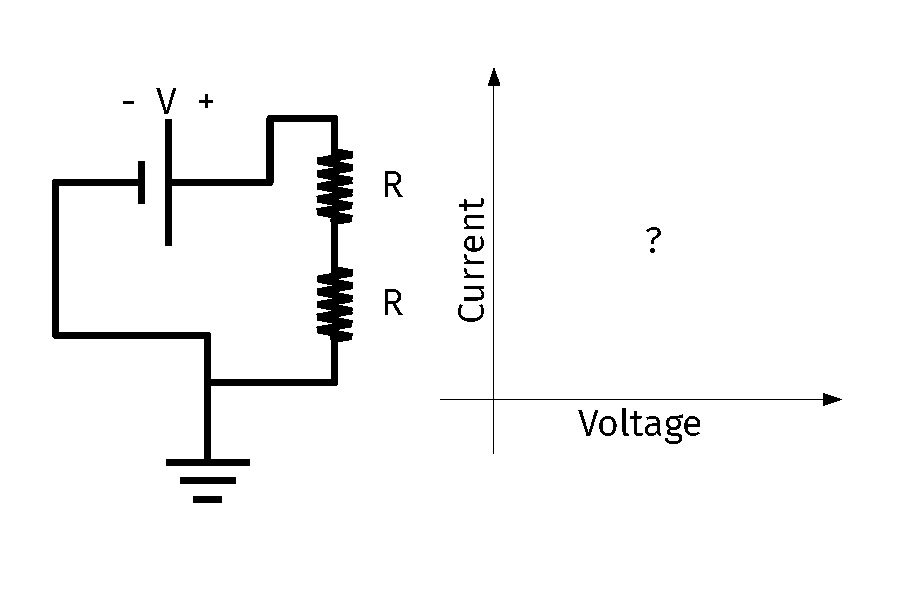
\includegraphics[width=\textwidth,trim=0.5cm 0cm 1cm 0cm,clip=true]{figures/iVCurve2.pdf}
\caption{\label{fig:iVCurve2} Circuits components are represented graphically by iV curves.}
\end{figure}
\end{column}
\begin{column}{0.5\textwidth}
\small
Should the slope now be greater than, less than, or equal to the that of Fig. \ref{fig:iVCurve1}?
\begin{itemize}
\item A: Greater than Fig. \ref{fig:iVCurve1}
\item B: Less than Fig. \ref{fig:iVCurve1}
\item C: Equal to Fig. \ref{fig:iVCurve1}
\item D: Cannot determine.
\end{itemize}
\end{column}
\end{columns}
\end{frame}

\begin{frame}{Current}
\begin{columns}[T]
\begin{column}{0.5\textwidth}
\begin{figure}
\centering
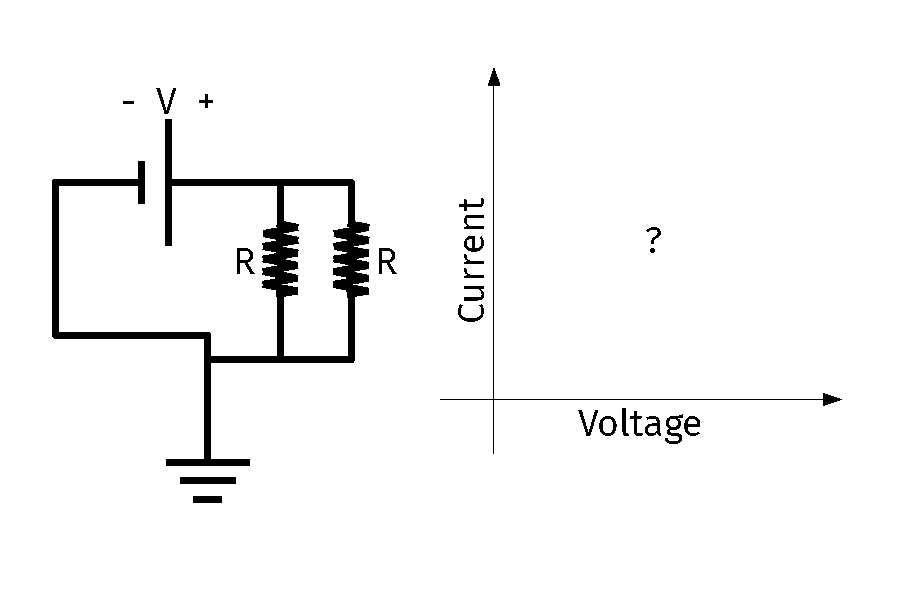
\includegraphics[width=\textwidth,trim=0.5cm 0cm 1cm 0cm,clip=true]{figures/iVCurve3.pdf}
\caption{\label{fig:iVCurve3} Circuits components are represented graphically by iV curves.}
\end{figure}
\end{column}
\begin{column}{0.5\textwidth}
\small
Should the slope now be greater than, less than, or equal to the that of Fig. \ref{fig:iVCurve1}?
\begin{itemize}
\item A: Greater than Fig. \ref{fig:iVCurve1}
\item B: Less than Fig. \ref{fig:iVCurve1}
\item C: Equal to Fig. \ref{fig:iVCurve1}
\item D: Cannot determine.
\end{itemize}
\end{column}
\end{columns}
\end{frame}

\begin{frame}{Current}
\begin{columns}[T]
\begin{column}{0.5\textwidth}
\begin{figure}
\centering
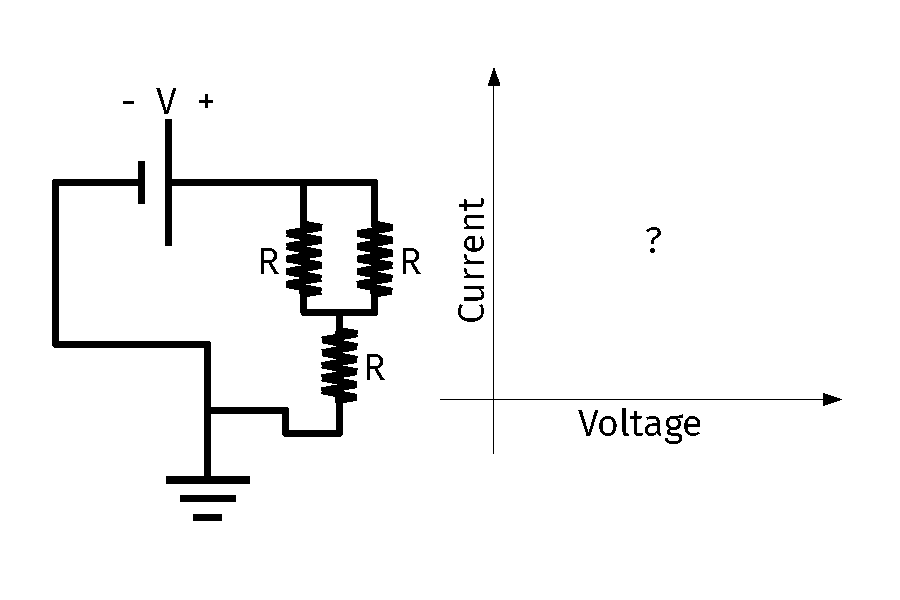
\includegraphics[width=\textwidth,trim=0.5cm 0cm 1cm 0cm,clip=true]{figures/iVCurve4.pdf}
\caption{\label{fig:iVCurve4} Circuits components are represented graphically by iV curves.}
\end{figure}
\end{column}
\begin{column}{0.5\textwidth}
\small
Should the slope now be greater than, less than, or equal to the that of Fig. \ref{fig:iVCurve1}?
\begin{itemize}
\item A: Greater than Fig. \ref{fig:iVCurve1}
\item B: Less than Fig. \ref{fig:iVCurve1}
\item C: Equal to Fig. \ref{fig:iVCurve1}
\item D: Cannot determine.
\end{itemize}
\end{column}
\end{columns}
\end{frame}

\begin{frame}{Current}
A \textit{fuse} is a device that disconnects a circuit if the current rises above a pre-defined value.  Some fuses have a wire that is rated to melt at a given current such that the circuit is no longer closed.  Suppose a deviced rated to consume 50 W is connected to a 12 V battery, in series with a fuse that is rated to blow at 1 A.  Does it blow?
\begin{itemize}
\item A: Yes
\item B: No
\item C: WAT
\end{itemize}
\end{frame}

\begin{frame}{Current}
Suppose a deviced rated to consume 50 W is connected to a 12 V battery, in series with a fuse that is rated to blow at 1 A.  Does it blow?
\begin{itemize}
\item A: Yes
\item B: No
\item C: WAT
\end{itemize}
\end{frame}

\begin{frame}{Current}
Suppose a deviced rated to consume 50 W is connected to a 12 V battery, in series with a fuse that is rated to blow at 5 A.  Does it blow?
\begin{itemize}
\item A: Yes
\item B: No
\item C: WAT
\end{itemize}
\end{frame}

\begin{frame}{Current}
Suppose a deviced rated to consume 50 W is connected to a 12 V battery, and a second identical device is connected in parallel to it.  In series with these devices and the battery is a fuse that is rated to blow at 5 A.  Does it blow?
\begin{itemize}
\item A: Yes
\item B: No
\item C: WAT
\end{itemize}
\end{frame}

\section{Nerve Signals}

\begin{frame}{Nerve Signals}
\begin{figure}
\centering
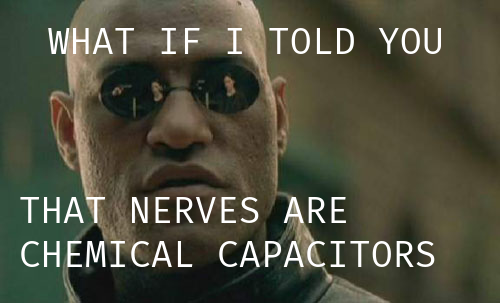
\includegraphics[width=0.9\textwidth]{figures/Matrix-Morpheus.png}
\end{figure}
\end{frame}

\begin{frame}{Nerve Signals}
\begin{figure}
\centering
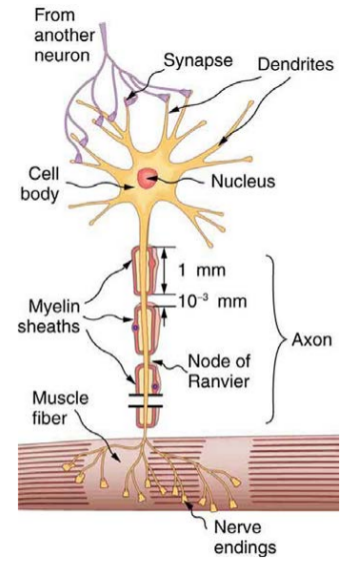
\includegraphics[width=0.3\textwidth]{figures/nerve1.png}
\caption{\label{fig:nerve1}  Structure of particular nerve cells known as \textit{axons}, which have 1 mm long sections of \textit{myelin} insulation, and $10^{-3}$ mm nodes.  Nerve signals are measured to propagate at 100 m/s in some cases.  No myelin means slower propagation.}
\end{figure}
\end{frame}

\begin{frame}{Nerve Signals}
\begin{figure}
\centering
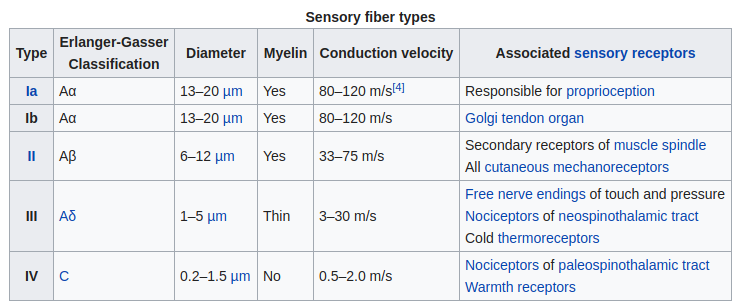
\includegraphics[width=0.8\textwidth]{figures/SensoryWiki.png}
\caption{\label{fig:sense} Lack of myelin allows cross-talk, but also slows down signals by a factor of 100.}
\end{figure}
\url{https://en.wikipedia.org/wiki/Nerve_conduction_velocity}
\end{frame}

\begin{frame}{Nerve Signals}
\begin{figure}
\centering
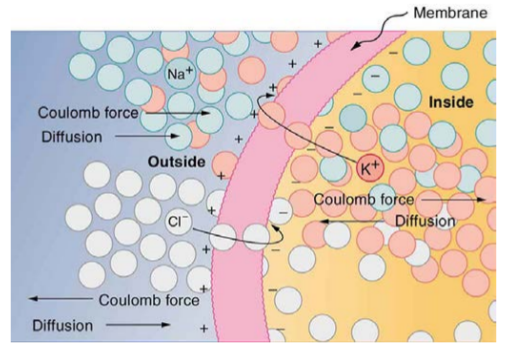
\includegraphics[width=0.7\textwidth]{figures/nerve2.png}
\caption{\label{fig:nerve2} The sodium-potassium pump is responsible for creating an action potential that propagates along a nerve fiber.  But how does this actually work?}
\end{figure}
\end{frame}

\begin{frame}{Nerve Signals}
We have a PhET simulation that demonstrates the mechanics of the pump. \\ \vspace{1cm}
\url{https://phet.colorado.edu/en/simulation/neuron}
\begin{enumerate}
\item Click stimulate to cause a propagating pulse.
\item Click potential chart to see the voltage versus time, called the \textit{action potential.}
\item Zoom in to the channels on the nerve membrane.  Which chemical elements cross the membrane, and when?
\end{enumerate}
\end{frame}

\begin{frame}{Nerve Signals}
\begin{figure}
\centering
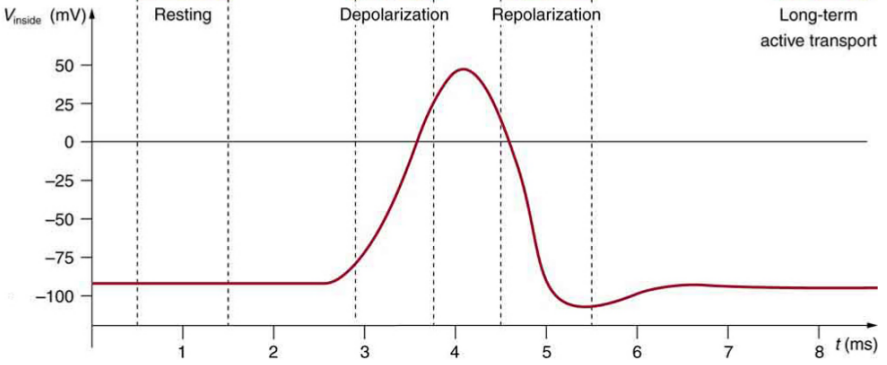
\includegraphics[width=0.8\textwidth]{figures/nerve3.png}
\caption{\label{fig:nerve3} We understand now how our nerves create this action potential, but there is a problem: \textbf{it is not fast enough.}}
\end{figure}
\end{frame}

\begin{frame}{Nerve Signals}
\begin{figure}
\centering
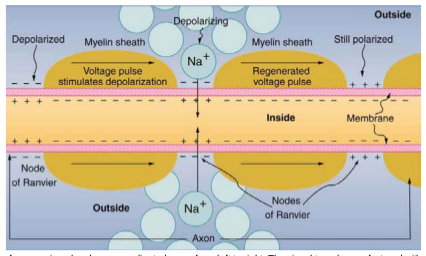
\includegraphics[width=0.5\textwidth]{figures/nerve5.png}
\caption{\label{fig:nerve4} The \textit{nodes of Ranvier} between \textit{myelin sheaths} create a system which propagates the signal without losing speed.}
\end{figure}
\small
\textbf{Professor calculation:} \textit{Let the speed of a signal in myelinated region be $v_{\rm m}$, and the speed in the node $v_{\rm n}$. Similarly, let the length of the myelinated area be $\Delta l_{\rm m}$, and that of the node be $\Delta l_{\rm n}$.  For a total nerve length $L$ that propagates a signal in time $T$, derive an expression for the speed of the signal, given $N$ nodes.}
\end{frame}

\begin{frame}{Nerve Signals}
\begin{figure}
\centering
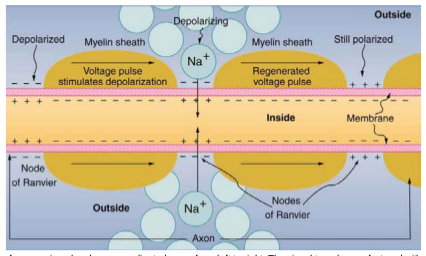
\includegraphics[width=0.5\textwidth]{figures/nerve5.png}
\caption{\label{fig:nerve4a} The \textit{nodes of Ranvier} between \textit{myelin sheaths} create a system which propagates the signal without losing speed.}
\end{figure}
\small
\begin{align}
L &= N(\Delta l_{\rm m} + \Delta l_{\rm n}) \\
T &= T(\Delta t_{\rm m} + \Delta t_{\rm n}) \\ 
v &= \frac{L}{T} = \frac{\Delta l_{\rm m} + \Delta l_{\rm n}}{\Delta t_{\rm m} + \Delta t_{\rm n}}
\end{align}
\end{frame}

\begin{frame}{Nerve Signals}
\begin{figure}
\centering
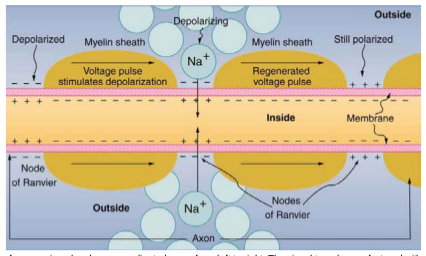
\includegraphics[width=0.5\textwidth]{figures/nerve5.png}
\caption{\label{fig:nerve4b} The nodes are small, the sheaths are large.}
\end{figure}
\small
\begin{align}
v &= \frac{L}{T} = \frac{\Delta l_{\rm m} + \Delta l_{\rm n}}{\Delta t_{\rm m} + \Delta t_{\rm n}} \\
\epsilon &= \frac{\Delta l_{\rm n}}{\Delta l_{\rm m}} ~~~ \kappa = \frac{v_{\rm m}}{v_{\rm n}} \\
v &= v_{\rm m} \left( \frac{1+\epsilon}{1+\kappa\epsilon} \right)
\end{align}
\end{frame}

\begin{frame}{Nerve Signals}
Now, we know that $\epsilon \approx 10^{-3}$ and $\kappa \approx 10^2$, so $\kappa\epsilon \approx 10^{-1}$.  We can approximate the final expression as
\begin{equation}
\boxed{
v \approx v_{\rm m} \left( 1-\kappa\epsilon + (\kappa\epsilon)^2 \right)
}
\end{equation}
Using $\kappa \approx 100$ and $\epsilon \approx 1/1000$, we get $v = 91\% v_{\rm m}$.
\begin{itemize}
\item Our nerves have evolved to have the smallest nodes possible so that we get the highest nerve speed possible
\item But we need the nodes to repolarize, otherwise the $IR$ drop would dissipate the signal (think of electrical grid)
\end{itemize}
\url{https://en.wikipedia.org/wiki/Nerve_conduction_velocity}
\end{frame}

\section{Conclusion}

\begin{frame}{Unit 2 Summary}
\textbf{Reading: Chapters 20 and 21}
\begin{enumerate}
\item Current, Ohm's Law, resistors and conductors
\item DC circuits I
\item Nerve signals
\item \alert{DC circuits II}
\end{enumerate}
\end{frame}

\section{Answers}

\begin{frame}{Answers}
\tiny
\begin{columns}[T]
\begin{column}{0.5\textwidth}
\begin{itemize}
\item $5 \times 10^{20}$ C
\item $8.34 \times 10^{28}$ free electrons per m$^3$
\item $10^{-4}$ m/s, or 0.1 mm/s
\item about 10 m$\Omega$
\item about 30 mV
\item about 300 mV
\item 12 m$\Omega$
\item 420 mA
\item $2 \times 10^{14}$
\item 1 keV
\item $2 \times 10^{17}$ eV
\item The slope on the graph will decrease
\item Less than Fig. \ref{fig:iVCurve1}
\item Greater than Fig. \ref{fig:iVCurve1}
\item Less than Fig. \ref{fig:iVCurve1}
\end{itemize}
\end{column}
\begin{column}{0.5\textwidth}
\begin{itemize}
\item Yes
\item No
\item Yes
\end{itemize}
\end{column}
\end{columns}
\end{frame}

\end{document}
